\documentclass[11pt]{article}
\usepackage[a4paper, margin=1.5cm]{geometry}
\usepackage[utf8]{inputenc}
\usepackage{babel}
\usepackage[spanish]{layout}
\usepackage[article]{ragged2e}
\usepackage{textcomp}
\usepackage{amsmath}
\usepackage{amssymb}
\usepackage{amsfonts}
\usepackage{proof}
\usepackage{enumerate}
\usepackage{graphicx}
\usepackage{multirow}

\setlength{\parindent}{0pt}

\title{
    Entrega 3 \\
    \large Sistemas Operativos II}
\author{Mellino, Natalia \and Farizano, Juan Ignacio}
\date{}

\begin{document}
\maketitle

\noindent\rule{\textwidth}{1pt}

\section*{Ejercicio 1}

Los procesos alternan entre ráfagas (o \emph{bursts}) en las que realizan cómputo interno
y otras, en donde están limitados por operaciones de entrada/salida (\emph{I/O bound}). 
En estos últimos la atención del planificador desaparece ya que el proceso deja de
estar \textbf{listo} y pasa a estar \textbf{bloqueado}. Entonces, si bien los procesos están en ejecución un largo período de tiempo estos
son tratados como procesos cortos porque al estar en una ráfaga de I/O, tienden
a estar bloqueados esperando a eventos (como los procesos interactivos) y en consecuencia,
requieren atención meramente ocasional del procesador permitiendo que mientras estos
procesos estén bloqueados se puedan ejecutar otros. \\

Un proceso largo es aquel que por mucho tiempo ha estado 'listo' o 'en ejecución', es decir,
un proceso que está en una larga ráfaga limitada por la CPU. Un ejemplo de proceso
largo puede ser el kernel del sistema operativo.


\section*{Ejercicio 2}

\subsection*{Apartado a)}

\begin{figure}[h!]
    \begin{center}
      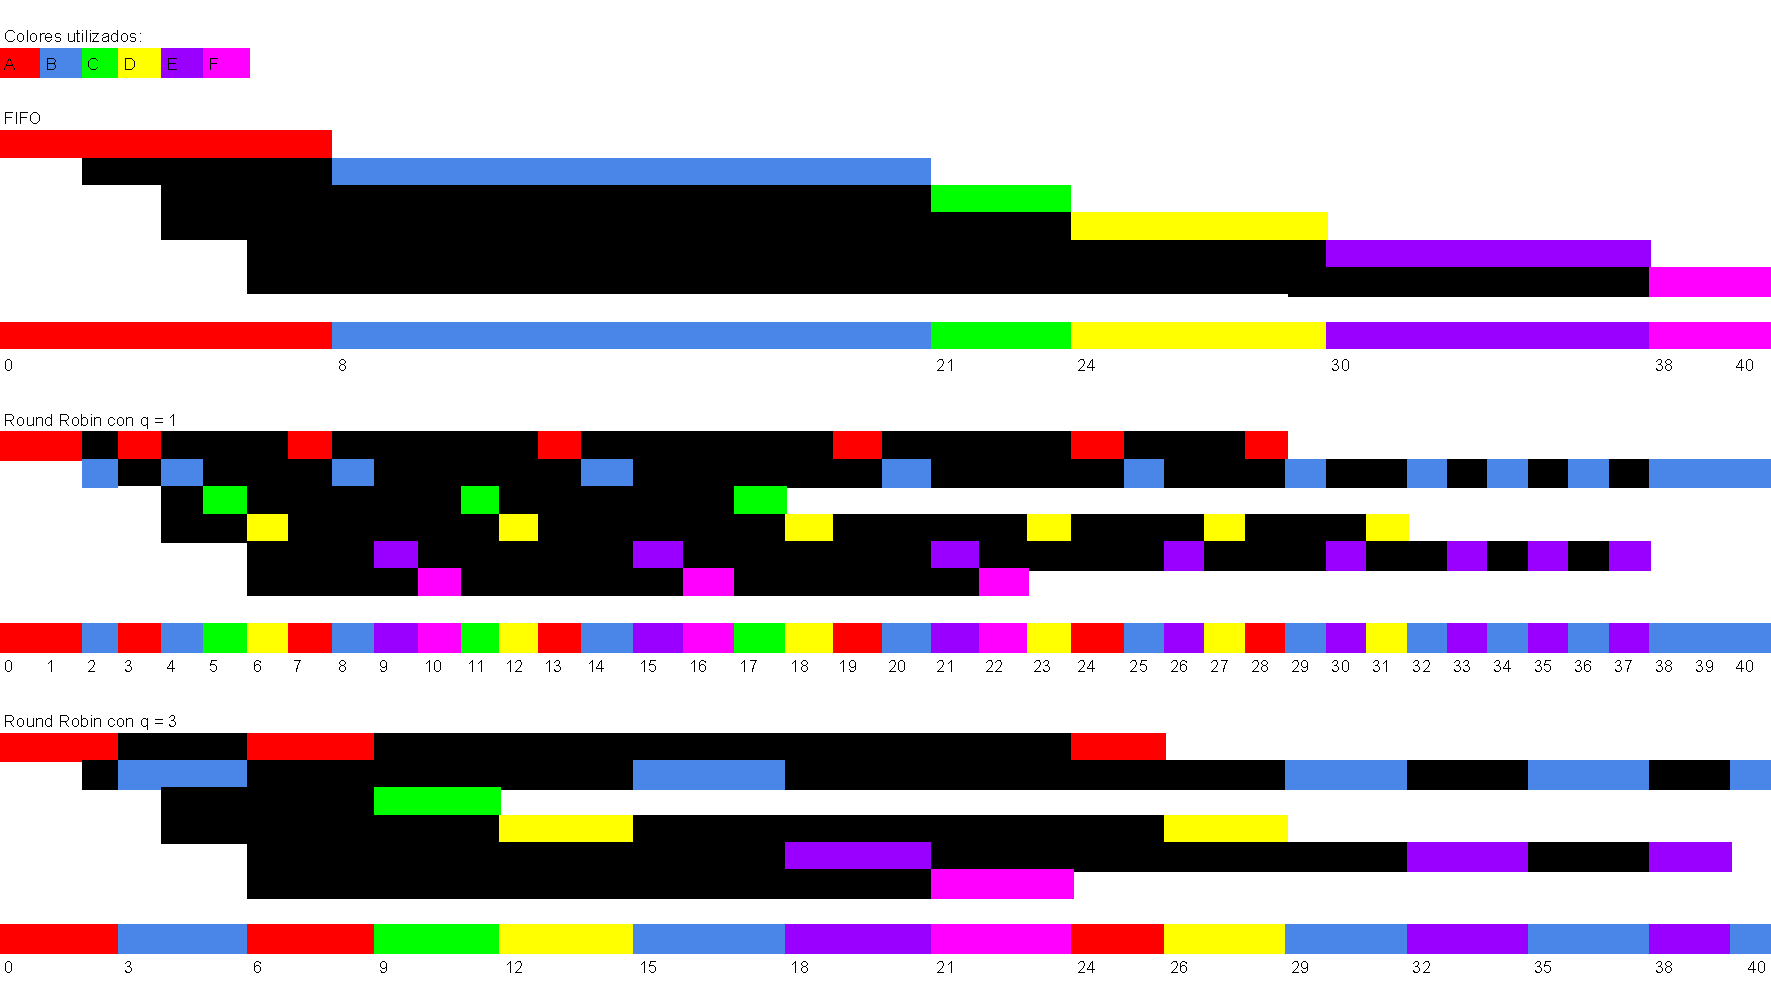
\includegraphics[width=\linewidth]{Graficos.pdf}
    \end{center}
  \end{figure}

\subsubsection*{Esquema FIFO}

\begin{center}
\begin{tabular}{|c|c|c|c|c|c|c|c|}
    \hline
    Proceso & Llegada & $t$ & Inicio & Fin & T & E & P \\
    \hline
    A & 0 & 8 & 0 & 8 & 8 & 0 & 1 \\
    \hline
    B & 2 & 13 & 8 & 21 & 19 & 6 & 1.46 \\
    \hline
    C & 4 & 3 & 21 & 24 & 20 & 17 & 6.6 \\
    \hline
    D & 4 & 6 & 24 & 30 & 26 & 20 & 4.3 \\
    \hline
    E & 6 & 8 & 30 & 38 & 32 & 24 & 4 \\
    \hline
    F & 6 & 3 & 38 & 41 & 35 & 32 & 11.6 \\ 
    \hline
    Promedio & & 6.83 & & & 23.3 & 16.5 & 4.82 \\
    \hline
\end{tabular}
\end{center}

\subsubsection*{Ronda con q = 1}

\begin{center}
    \begin{tabular}{|c|c|c|c|c|c|c|c|}
        \hline
        Proceso & Llegada & $t$ & Inicio & Fin & T & E & P \\
        \hline
        A & 0 & 8 & 0 & 28 & 28 & 20 & 3.5 \\
        \hline
        B & 2 & 13 & 2 & 40 & 38 & 25 & 2.92 \\
        \hline
        C & 4 & 3 & 5 & 17 & 13 & 10 & 4.33 \\
        \hline
        D & 4 & 6 & 6 & 31 & 27 & 21 & 4.5 \\
        \hline
        E & 6 & 8 & 9 & 37 & 31 & 23 & 3.87 \\
        \hline
        F & 6 & 3 & 10 & 21 & 15 & 12 & 5 \\ 
        \hline
        Promedio & & 6.83 & & & 25.3 & 18.5 & 4.02  \\
        \hline
    \end{tabular}
\end{center}

\subsubsection*{Ronda con q = 3}

\begin{center}
    \begin{tabular}{|c|c|c|c|c|c|c|c|}
        \hline
        Proceso & Llegada & $t$ & Inicio & Fin & T & E & P \\
        \hline
        A & 0 & 8 & 0 & 25 & 25 & 17 & 3.12 \\
        \hline
        B & 2 & 13 & 2 & 40 & 38 & 25 & 2.92 \\
        \hline
        C & 4 & 3 & 8 & 11 & 7 & 4 & 2.33 \\
        \hline
        D & 4 & 6 & 11 & 28 & 24 & 18 & 4 \\
        \hline
        E & 6 & 8 & 17 & 39 & 33 & 25 & 4.12 \\
        \hline
        F & 6 & 3 & 20 & 23 & 17 & 14 & 5.66 \\ 
        \hline
        Promedio & & 6.83 & & & 24 & 17.16 & 3.69 \\
        \hline
    \end{tabular}
\end{center}

\subsection*{Apartado b)}

Conclusiones:

\begin{itemize}
    \item La ronda con q = 3 destaca por ser la que menor
          penalización posee en promedio.
    \item El método FIFO se destaca por tener el menos tiempo de espera en promedio
          y el menor tiempo desde que un proceso llega a su fin. 
\end{itemize}

\end{document}